\section{Vertex Locator (VELO)}

%=========================================================================%
%=============================  Vertex reconstruction  ==========================%
%=========================================================================%
%The properties of these decays such as the decay position, lifetime of the B/D mesons and their  products need also to be highly accurate in order to minimise the uncertainty on the key measurements at the LHCb experiment.  
%Particle interactions are characterised by particles originating from a common point in space. With the presence of interacting particles In the case of particle production or with the association of a single parent particle in interactions involving decays.
%
%Since the focus of the LHCb experiment is the observation of rare decays it follows that the detector be optimised such that 
%
%The position of beam proton-proton interactions and particle decays are described by a vertex. A vertex provides information on the position of the event and the particles produced as a result. The identification, positional accuracy of vertices along with the correct association of interactions to their product particles is fundamental in achieving the physics goals of the LHCb experiment, its presence in an event serves as a clear indicator of the rare physics processes that are the focus of the LHCb detector. 
%
%Unique to the LHCb detector.
%
%Vertex reconstruction of interaction points and decay vertices is an extremely important aspect of the LHCb experiment. This is due to the primary focus of the experiment being around the analysis of rare decay processes. From this is follows that the LHCb detector must have good tracking around the interaction region such that a vertex which has been inferred from the direction of the tracks has a small error on its position and i.e. decay lifetime. In addition to this accurate tracking is required in order to accurately measure the impact parameter of tracks, an important input for the trigger.

%Particle interactions are characterised by particles originating from a common point in space. With the presence of interacting particles In the case of particle production or with the association of a single parent particle in interactions involving decays.
%
%Since the focus of the LHCb experiment is the observation of rare decays it follows that the detector be optimised such that 
%
%The position of beam proton-proton interactions and particle decays are described by a vertex. A vertex provides information on the position of the event and the particles produced as a result. The identification, positional accuracy of vertices along with the correct association of interactions to their product particles is fundamental in achieving the physics goals of the LHCb experiment, its presence in an event serves as a clear indicator of the rare physics processes that are the focus of the LHCb detector. 
%
%Unique to the LHCb detector.
%
%Vertex reconstruction of interaction points and decay vertices is an extremely important aspect of the LHCb experiment. This is due to the primary focus of the experiment being around the analysis of rare decay processes. From this is follows that the LHCb detector must have good tracking around the interaction region such that a vertex which has been inferred from the direction of the tracks has a small error on its position and i.e. decay lifetime. In addition to this accurate tracking is required in order to accurately measure the impact parameter of tracks, an important input for the trigger.
%To achieve this the LHCb detector has a dedicated vertex reconstruction sub-detector called the VELO detector. The VELO detector is made up of a series of silicon stations which are positioned along the direction of the beam (Fig \ref{fig: VELO_silicon_stations}). Each station is segmented into two halves such that the two halves of the VELO can through a mechanical system move into open and closed configurations(Fig \ref{fig: VELO layout}).
%
%This mechanism enables the VELO detector to maximise its resolution by minimising the distance between the nominal interaction region and the sensitive areas of the VELO. During periods of stable beam the minimum distance between the nominal interaction region and the sensitive area of the VELO detector is $ \approx 5mm$. However during the process of beam injection the width of the beam can be greater. To protect the components of the VELO during this process the two halves of the VELO are separated by as much as $6mm$.

%\begin{itemize}
%	\item Station layout
%	\item r-$\phi$ sensors
%	\item pile-up sensors and L0 trigger
%	\item LHC vacuum and VELO vacuum
%	\item RF foils
%\end{itemize}

%1. VELO motivation
%2. VELO features and layout
%3. VELO performance

The detection of rare B and D meson decays is a key requirement to meet the physics goals of the LHCb experiment.  In the LHCb detector these processes are characterised by the presence of production and decay vertices. To maximise the sensitivity of detecting and correctly identifying these events a dedicated sub-detector system called the VELO (Vertex locator) is employed around the nominal interaction region.

The VELO is made up of two halves (left and right) which open and close about the interaction region depending on the status of the LHC beam (see fig \ref{fig: VELO layout}). During the beam fill or dumping the VELO is put into its open configuration in order to minimise radiation damage to its components. When the beam is stable and appropriate for physics data taking the VELO is put into it closed position (In this configuration the minimal distance between the silicon trackers and the beamline is 8mm) to maximise its tracking resolution. Each half contains 21 silicon tracking stations positioned at different points along the direction of the beamline. The tracking stations are approximately semi-circular in shape, 300 \,$\mu$m thick and composed of R and $\phi$ sensors. The angular coverage of the VELO detector can be seen in figure \ref{fig: velo angular acceptance}.

The VELO reconstructs vertices with a resolution of $\sim10\,\mu$m; this corresponds to a $\sim40$ fs resolution in the measurement of particle lifetimes and an impact parameter resolution of $20\,\mu$m. %Reconstructs particles from $15$ mrad to $390$ mrad.
\begin{figure}
	\centering
	\includegraphics[width=0.5\columnwidth]{/Users/admin/Dropbox/LHCb/detector/VELO/images/silicon_stations.jpg}
	\caption{VELO silicon stations during partial construction of the VELO sub-detector}
	\label{fig: VELO_silicon_stations}
\end{figure}

\begin{figure}
	\centering
	\includegraphics[width=\columnwidth]{/Users/admin/Dropbox/LHCb/detector/VELO/images/VELO_open_closed.png}
	\caption{The front face of the first modules is also illustrated in both the closed and open configurations}
	\label{fig: VELO layout}
\end{figure}

\begin{figure}
	\centering
	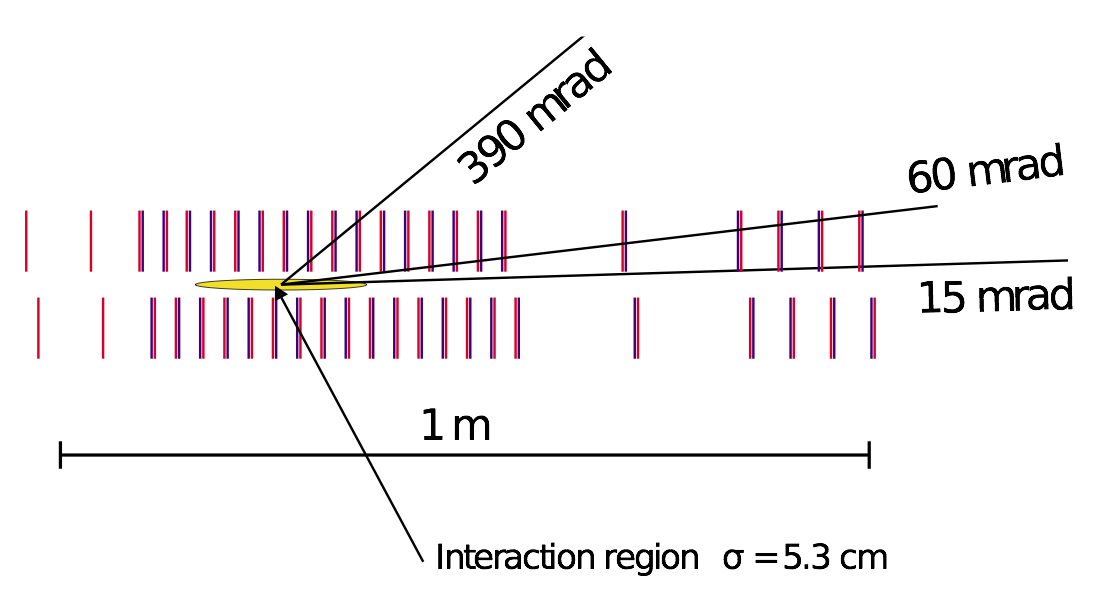
\includegraphics[width=0.7\columnwidth]{Chapters/detector/images/velo_angular_acceptance.png}
	\caption{The layout of the VELO R (red) and $\phi$ (blue) sensors shown in the (x,z) plane. A $\pm2\sigma$ area around the nominal interaction point is shown in yellow. Lines drawn at 390 mrad and 15 mrad represent the maximum and minimum angular coverage, while the line at 60 mrad shows the average track angle in minimum bias events. The left-most two pairs of R sensors are the pileup veto stations.}
	\label{fig: velo angular acceptance}
\end{figure}


\begin{figure}
	\centering
	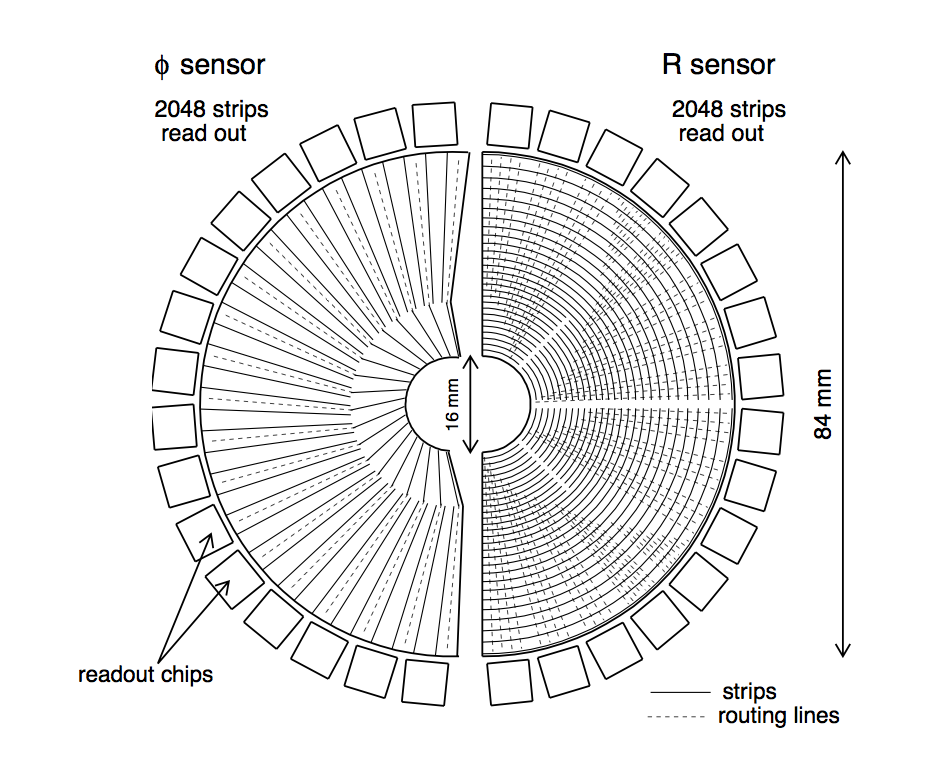
\includegraphics[width=0.5\columnwidth]{Chapters/detector/images/r-phi_sensors.png}
	\caption{Schematic diagram of an R sensor (right) and a $\phi$ sensor (left)}
	\label{fig: r-phi sensors}
\end{figure}